%%%%%%%% ICML 2023 EXAMPLE LATEX SUBMISSION FILE %%%%%%%%%%%%%%%%%

\documentclass{article}

% Recommended, but optional, packages for figures and better typesetting:
\usepackage{microtype}
\usepackage{graphicx}
\usepackage{subfigure}
\usepackage{booktabs} % for professional tables


\usepackage{tikz}
% Corporate Design of the University of Tübingen
% Primary Colors
\definecolor{TUred}{RGB}{165,30,55}
\definecolor{TUgold}{RGB}{180,160,105}
\definecolor{TUdark}{RGB}{50,65,75}
\definecolor{TUgray}{RGB}{175,179,183}

% Secondary Colors
\definecolor{TUdarkblue}{RGB}{65,90,140}
\definecolor{TUblue}{RGB}{0,105,170}
\definecolor{TUlightblue}{RGB}{80,170,200}
\definecolor{TUlightgreen}{RGB}{130,185,160}
\definecolor{TUgreen}{RGB}{125,165,75}
\definecolor{TUdarkgreen}{RGB}{50,110,30}
\definecolor{TUocre}{RGB}{200,80,60}
\definecolor{TUviolet}{RGB}{175,110,150}
\definecolor{TUmauve}{RGB}{180,160,150}
\definecolor{TUbeige}{RGB}{215,180,105}
\definecolor{TUorange}{RGB}{210,150,0}
\definecolor{TUbrown}{RGB}{145,105,70}

% hyperref makes hyperlinks in the resulting PDF.
% If your build breaks (sometimes temporarily if a hyperlink spans a page)
% please comment out the following usepackage line and replace
% \usepackage{icml2023} with \usepackage[nohyperref]{icml2023} above.
\usepackage{hyperref}


% Attempt to make hyperref and algorithmic work together better:
\newcommand{\theHalgorithm}{\arabic{algorithm}}

\usepackage[accepted]{icml2023}

% For theorems and such
\usepackage{amsmath}
\usepackage{amssymb}
\usepackage{mathtools}
\usepackage{amsthm}
 
% if you use cleveref..
\usepackage[capitalize,noabbrev]{cleveref}

%%%%%%%%%%%%%%%%%%%%%%%%%%%%%%%%
% THEOREMS
%%%%%%%%%%%%%%%%%%%%%%%%%%%%%%%%
\theoremstyle{plain}
\newtheorem{theorem}{Theorem}[section]
\newtheorem{proposition}[theorem]{Proposition}
\newtheorem{lemma}[theorem]{Lemma}
\newtheorem{corollary}[theorem]{Corollary}
\theoremstyle{definition}
\newtheorem{definition}[theorem]{Definition}
\newtheorem{assumption}[theorem]{Assumption}
\theoremstyle{remark}
\newtheorem{remark}[theorem]{Remark}

% Todonotes is useful during development; simply uncomment the next line
%    and comment out the line below the next line to turn off comments
%\usepackage[disable,textsize=tiny]{todonotes}
\usepackage[textsize=tiny]{todonotes}


% The \icmltitle you define below is probably too long as a header.
% Therefore, a short form for the running title is supplied here:
\icmltitlerunning{Project Report Template for Data Literacy 2023/24}

\begin{document}

\twocolumn[
\icmltitle{My Data Literacy Project\\ (Replace this with your Project Title)}

% It is OKAY to include author information, even for blind
% submissions: the style file will automatically remove it for you
% unless you've provided the [accepted] option to the icml2023
% package.

% List of affiliations: The first argument should be a (short)
% identifier you will use later to specify author affiliations
% Academic affiliations should list Department, University, City, Region, Country
% Industry affiliations should list Company, City, Region, Country

% You can specify symbols, otherwise they are numbered in order.
% Ideally, you should not use this facility. Affiliations will be numbered
% in order of appearance and this is the preferred way.
\icmlsetsymbol{equal}{*}

\begin{icmlauthorlist}
\icmlauthor{Jana Hoffmann}{equal,first}
\icmlauthor{Julia Graf}{equal,second}
\icmlauthor{Jessie Midgley}{equal,third}
\icmlauthor{Tithi Rakshit}{equal,fourth}
\end{icmlauthorlist}

% fill in your matrikelnummer, email address, degree, for each group member
\icmlaffiliation{first}{Matrikelnummer 5760486, jana2.hoffmann@student.uni-tuebingen.de, MSc Bioinformatics}
\icmlaffiliation{second}{Matrikelnummer 5656882, jul.graf@student.uni-tuebingen.de, MSc Bioinformatics}
\icmlaffiliation{third}{Matrikelnummer 6620875, jessie.midgley@student.uni-tuebingen.de, MSc Bioinformatics}
\icmlaffiliation{fourth}{Matrikelnummer 6635972, tithi.rakshit@student.uni-tuebingen.de, MSc Quantitative Data Science}

% You may provide any keywords that you
% find helpful for describing your paper; these are used to populate
% the "keywords" metadata in the PDF but will not be shown in the document
\icmlkeywords{Machine Learning, ICML}

\vskip 0.3in
]

% this must go after the closing bracket ] following \twocolumn[ ...

% This command actually creates the footnote in the first column
% listing the affiliations and the copyright notice.
% The command takes one argument, which is text to display at the start of the footnote.
% The \icmlEqualContribution command is standard text for equal contribution.
% Remove it (just {}) if you do not need this facility.

%\printAffiliationsAndNotice{}  % leave blank if no need to mention equal contribution
\printAffiliationsAndNotice{\icmlEqualContribution} % otherwise use the standard text.

\begin{abstract}
Put your abstract here. Abstracts typically start with a sentence motivating why the subject is interesting. Then mention the data, methodology or methods you are working with, and describe results. 
\end{abstract}

\section{Introduction}\label{sec:intro}

The Oktoberfest, held annually in Munich, Germany, is one of the world's most renowned folk festivals, attracting millions annually. In this paper, we analyze nearly four decades of Oktoberfest data, spanning from 1985 to 2023, to uncover insights into its evolution and various influencing factors. Understanding the dynamics of this iconic event is not only of cultural significance but also holds economic and societal implications. \\
This paper is structured as follows: \Cref{sec:methods} outlines our data sources and analytical methods. \Cref{sec:results} presents our findings, elucidating key trends and correlations observed within the Oktoberfest dataset, and \Cref{sec:conclusion} discusses the implications of our findings and offers insights into future festivals.\\

\section{Data and Methods}\label{sec:methods}
The annual Oktoberfest data from 1985 to 2022 was retrieved from the Open Data Portal of the Statistical Office Munich. This dataset contains the yearly festival duration, visitor numbers, as well as consumption and prices for beer and roast chicken. Additional data for 2023 was retrieved from the State Capital Munich Portal. \\
We examine the evolution of visitor numbers over the years and use four additional datasets to investigate how these are influenced by precipitation. Weather datasets were retrieved from the Open Data Server of the German Meteorological Service (DWD) and contain data from the weather stations ``München-Stadt" and ``München (Bavariaring)". Two of the datasets contain the daily precipitation in millimeters, with one spanning from 1954 to 2022, and the other from 2022 to 2024~\citep{3}~\citep{4}. The remaining two datasets contain the hourly precipitation in millimeters, in ranges from 1997 to 2022, and from 2022 to 2024~\citep{1}~\citep{2}. We use the pearson correlation coefficient (PCC) to investigate the correlation between the average number of daily visitors and the average daily precipitation during each Oktoberfest, and also constrain daily precipitation between 10am and 10pm. The PCC ranges from -1 to 1, where a higher absolute value indicates a stronger correlation between two variables~\cite{thonield}.\\
\textcolor{red}{missing: heat map data}\\
We investigate visitor, price and consumption trends over the years, and use the PCC to explore the correlation between beer price and per capita beer consumption.To account for inflation over time, beer prices are also adjusted by the Consumer Price Index (CPI) which measures the monthly average price development of goods and services purchased by German households. The CPI data was collected from the Federal Statistical Office of Germany (Destatis).\\
\textcolor{red}{missing: price prediction}\\

% This is the template for a figure from the original ICML submission pack. In lecture 10 we will discuss plotting in detail.
% Refer to this lecture on how to include figures in this text.
% 
% \begin{figure}[ht]
% \vskip 0.2in
% \begin{center}
% \centerline{\includegraphics[width=\columnwidth]{icml_numpapers}}
% \caption{Historical locations and number of accepted papers for International
% Machine Learning Conferences (ICML 1993 -- ICML 2008) and International
% Workshops on Machine Learning (ML 1988 -- ML 1992). At the time this figure was
% produced, the number of accepted papers for ICML 2008 was unknown and instead
% estimated.}
% \label{icml-historical}
% \end{center}
% \vskip -0.2in
% \end{figure}

\section{Results}\label{sec:results}
\subsection*{3.1 Visitor trend over the years}
The visitor numbers fluctuate over the years, and we observe a dramatic drop in visitor numbers in the year 2001. The Oktoberfest was cancelled in 2020 and 2021 due to the pandemic. A new record number of visitors was set in 2023.\\
\textcolor{red}{add figure: visitor trends.}\\
\subsection*{3.2 Influence of precipitation on visitor numbers}
The PCC we for the mean daily visitors and the mean daily precipitation in each year is around -0.1913. The correlation is thus negative. As the amount of precipitation increases the amount of visitors decrease. Since the absolute value of the PCC is low but not zero the variables correlate but the correlation is weak. Due to the fact that the daily precipitation includes hours of the day were the Oktoberfest isn't open we also investigated if the mean precipitation at day time correlates with the amount of visitors stronger. We therefor considered the precipitation between 10am and 10pm. The PCC than is around -0.2276. So the correlation gets stronger but is still weak.
\begin{figure}[]% this figure made with
  % plt.rcParams.update(bundles.icml2022(column="half”,usetex=False))
  % fig,ax = plt.subplots(nrows=1, ncols=1)
  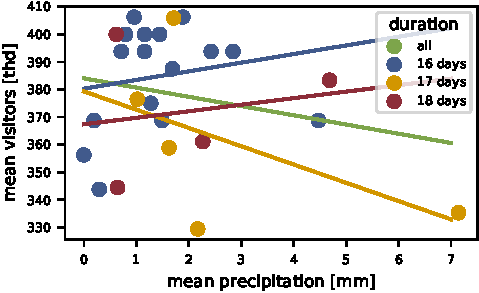
\includegraphics{fig/totalprecipitation.pdf}
  \caption{The mean daily visitors of the Oktoberfest as a function of the mean daily precipitation between 10am and 10pm at the time of the Oktoberfest in each year. The lines are the linear regression lines of the data points.}
  \label{figure_precipitation}
\end{figure}\\
\noindent
In Figure~\ref{figure_precipitation} we can see the weak negative correlation represented by the green regression line which has a negative gradient while the values at both axis increase. The regression line shows that the mean daily amount of visitors of the Oktoberfest decrease by around 25.000 people as the mean precipitation at day time increases from zero millimeters to seven.\\
\subsection*{3.3 Tourists to Upper Bavaria during Oktoberfest}
\subsection*{3.4 Price and consumption trends}
We see an almost linear increase in beer price over the years. The per capita consumption also shows an overall increase, but fluctuates over the years. We observe a low per capita beer consumption in 2023, likely due to to the record number of visitors that year. The correlation plot shows that beer consumption continues to increase, despite rising beer prices. This strong positive relationship between beer price and consumption is confimred by the PCC of .... \\
Adjusting beer prices by the CPI slightly increases the correlation between price and consumption from ... (excluding 2023 outlier) to ....\\
For roast chicken, the PCC coeffiecient of ... shows a strong negative correlation between price and consumption.
\subsection*{3.5 Beer price prediction}

\section{Discussion \& Conclusion}\label{sec:conclusion}
The sudden drop in visitors in 2001 could potentially be explained by the 9/11 terrorist attacks that occurred a few weeks prior to the festival. Perhaps surprisingly, visitor numbers were still very low during the first festival after the pandemic in 2022. This could be due to the public's remaining fears of contracting the virus in large crowds.\\


Since the PCC for the mean precipitation and the mean daily visitors is weak it looks like the precipitation doesn't influence the visitors of the Oktoberfest much.
The PCC is weak for the mean precipitation at day time and the mean daily vistors. This can have many reasons. One reason is, that we looked at the correlation of the mean over all days for each Oktoberfest and not at the correlation between the precipitation at each day and the visitor number of each day due to the lack of data. If in one year there is a very rainy day at which fewer people visit followed by good days with no rain were all the vistors come instead we couldn't see that the people that visited were influenced by the precipitation when only using the mean. Due to that even a weak correaltion shows that the amount of precipitation influences the amount of vistors. ........ In conclusion we can say, that the amount of precipitation influences the amount of visitors, but there are factors that influence the amount of precipitatioin more.\\

The rising beer prices do not have a negative effect on the beer consumption, as we observe a positive correlation between beer price and consumption per capita. The Oktoberfest has grown in popularity since 1985 and now also attracts many international tourists. This might explain why people are willing to spend more on a "Maß" beer, especially for some international tourists who might be used to paying the same prices in their home country. The 2023 Oktoberfest was the first to introduce free water fountains, which could have led to the decrease in overall beer consumption we see that year. Interestingly, the positive correlation in beer consumption and price is opposite to what we observed with the chicken data. However, the reason for the decrease in chicken consumption might have less to do with the increase in price, but rather with the rise in popularity of other foods.

\section*{Contribution Statement}

Explain here, in one sentence per person, what each group member contributed. For example, you could write: Max Mustermann collected and prepared data. Gabi Musterfrau and John Doe performed the data analysis. Jane Doe produced visualizations. All authors will jointly wrote the text of the report. Note that you, as a group, a collectively responsible for the report. Your contributions should be roughly equal in amount and difficulty.

\section*{Notes} 

Your entire report has a \textbf{hard page limit of 4 pages} excluding references. (I.e. any pages beyond page 4 must only contain references). Appendices are \emph{not} possible. But you can put additional material, like interactive visualizations or videos, on a githunb repo (use \href{https://github.com/pnkraemer/tueplots}{links} in your pdf to refer to them). Each report has to contain \textbf{at least three plots or visualizations}, and \textbf{cite at least two references}. More details about how to prepare the report, inclucing how to produce plots, cite correctly, and how to ideally structure your github repo, will be discussed in the lecture, where a rubric for the evaluation will also be provided.


\bibliography{bibliography}
\bibliographystyle{icml2023}

\end{document}


% This document was modified from the file originally made available by
% Pat Langley and Andrea Danyluk for ICML-2K. This version was created
% by Iain Murray in 2018, and modified by Alexandre Bouchard in
% 2019 and 2021 and by Csaba Szepesvari, Gang Niu and Sivan Sabato in 2022.
% Modified again in 2023 by Sivan Sabato and Jonathan Scarlett.
% Previous contributors include Dan Roy, Lise Getoor and Tobias
% Scheffer, which was slightly modified from the 2010 version by
% Thorsten Joachims & Johannes Fuernkranz, slightly modified from the
% 2009 version by Kiri Wagstaff and Sam Roweis's 2008 version, which is
% slightly modified from Prasad Tadepalli's 2007 version which is a
% lightly changed version of the previous year's version by Andrew
% Moore, which was in turn edited from those of Kristian Kersting and
% Codrina Lauth. Alex Smola contributed to the algorithmic style files.
